\clearpage
\subsection{Mandelbrot set}
\label{Mandelbrot_demo}

\epigraph{You know, if you magnify the coastline, it still looks like
a coastline, and a lot of other things have this property. Nature has
recursive algorithms that it uses to generate clouds and Swiss cheese
and things like that.}
{Donald Knuth, interview (1993)}

Mandelbrot set is a fractal, which exhibits self-similarity.

When you increase scale, you see that this characteristic pattern repeating infinitely.

Here is a demo\footnote{Download it \href{http://go.yurichev.com/17306} {here},} 
written by \q{Sir\_Lagsalot} in 2009, that draws 
the Mandelbrot set, which is just a x86 program with executable file size of only 64 bytes.
There are only 30 16-bit x86 instructions.

Here it is what it draws:

\begin{figure}[H]
\centering
\myincludegraphics{examples/demos/mandelbrot/1.png}
\end{figure}

Let's try to understand how it works.

\subsubsection{Theory}

\myparagraph{A word about complex numbers}

A complex number is a number that consists of two parts---real (Re) and imaginary (Im).


The complex plane is a two-dimensional plane where any complex number can be placed: the real part is one coordinate
and the imaginary part is the other.

Some basic rules we have to keep in mind:

\begin{itemize}
\item Addition: $(a+bi) + (c+di) = (a+c) + (b+d)i$

In other words:

$\operatorname{Re}(sum) = \operatorname{Re}(a) + \operatorname{Re}(b)$

$\operatorname{Im}(sum) = \operatorname{Im}(a) + \operatorname{Im}(b)$

\item Multiplication: $(a+bi) (c+di) = (ac-bd) + (bc+ad)i$

In other words:

$\operatorname{Re}(product) = \operatorname{Re}(a) \cdot \operatorname{Re}(c) - \operatorname{Re}(b) \cdot \operatorname{Re}(d)$

$\operatorname{Im}(product) = \operatorname{Im}(b) \cdot \operatorname{Im}(c) + \operatorname{Im}(a) \cdot \operatorname{Im}(d)$

\item Square: $(a+bi)^2 = (a+bi) (a+bi) = (a^2-b^2) + (2ab)i$

In other words:

$\operatorname{Re}(square) = \operatorname{Re}(a)^2-\operatorname{Im}(a)^2$

$\operatorname{Im}(square) = 2 \cdot \operatorname{Re}(a) \cdot \operatorname{Im}(a)$

\end{itemize}

\myparagraph{How to draw the Mandelbrot set}

The Mandelbrot set is a set of points for which the $z_{n+1} = {z_n}^2 + c$ recursive sequence
(where $z$ and $c$ are complex numbers and $c$ 
is the starting value)
does not approach infinity.\\
\\
In plain English language: 

\begin{itemize}
\item Enumerate all points on screen. 
\item Check if the specific point 
is in the Mandelbrot set.
\item Here is how to check it:

  \begin{itemize}
  \item Represent the point as a complex number.
  \item Calculate the square of it.
  \item Add the starting value of the point to it.
  \item Does it go off limits? If yes, break.
  \item Move the point to the 
new place at the coordinates we just calculated.
  \item Repeat all this for some reasonable 
number of iterations.
  \end{itemize}

\item The point is still in limits?
Then draw the point.

\item The point has eventually gone off limits?

  \begin{itemize}
    \item (For a black-white image) do not draw anything.
    \item 

(For a colored image) transform the number of iterations to some color. 
      So the color shows the speed with which point has gone off limits.
  \end{itemize}

\end{itemize}

%
Here is Pythonesque algorithm for both complex and integer number representations:

\lstinputlisting[caption=For complex numbers]{examples/demos/mandelbrot/algo_cplx_EN.lst}


The integer version is where the operations on complex numbers are replaced with integer operations according to the rules
which were explained above.

\lstinputlisting[caption=For integer numbers]{examples/demos/mandelbrot/algo_int_EN.lst}

Here is also a C\# source 
which is present in the Wikipedia article\footnote{\href{http://go.yurichev.com/17307}{wikipedia}}, but we'll modify it
so it will print the iteration numbers instead of some symbol
\footnote{Here is also the executable file: 
\href{http://go.yurichev.com/17163}{beginners.re}}:

\lstinputlisting{examples/demos/mandelbrot/dump_iterations.cs}

Here is the resulting file, 
which is too wide to be included here: \\
\href{http://go.yurichev.com/17164}{beginners.re}.

The maximal number of iterations is 40, so when you see 40 in this dump, it means that this point has been wandering
for 40 iterations but never got off limits. 

A number $n$ less then 40 mean that point remained inside the bounds only for $n$ iterations, 
then it went outside them.

\clearpage
There is a cool demo available at 
\url{http://go.yurichev.com/17309}, which shows
visually how the point moves on the plane at each iteration for some specific point. 
Here are two screenshots.

%
First, we've clicked inside the yellow area and saw that the trajectory (green line)
eventually swirls at some point inside:

\begin{figure}[H]
\centering
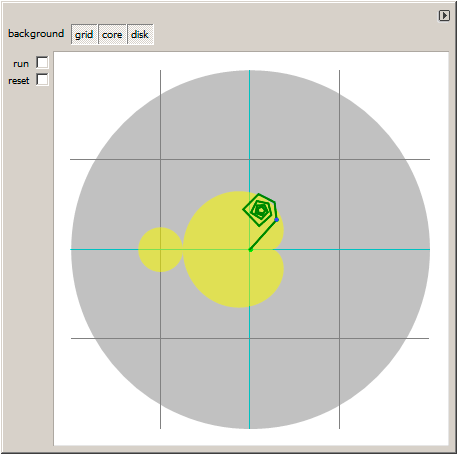
\includegraphics[width=0.7\textwidth]{examples/demos/mandelbrot/demo1.png}
\caption{Click inside yellow area}
\end{figure}


This implies that the point we've clicked belongs to the Mandelbrot set.

\clearpage

Then we've clicked outside the yellow area and saw a much more chaotic point movement, 
which quickly went off bounds:

\begin{figure}[H]
\centering
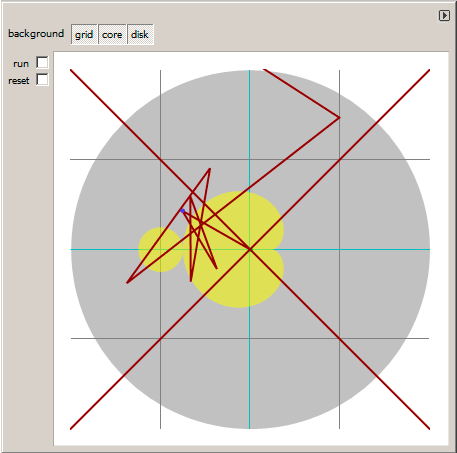
\includegraphics[width=0.7\textwidth]{examples/demos/mandelbrot/demo2.png}
\caption{Click outside yellow area}
\end{figure}

This mean the point not belongs 
to Mandelbrot set.

Another good demo is available here: 
\url{http://go.yurichev.com/17310}.

\clearpage
\subsubsection{Let's get back to the demo}


The demo, although very tiny (just 64 bytes or 30 instructions), implements the common algorithm 
described here, but using some coding tricks.

%
The source code is easily downloadable, so here is it, but let's also add comments:

\lstinputlisting[caption=Commented source code,numbers=left]{examples/demos/mandelbrot/Microbrot_commented_EN.asm}

Algorithm:

\begin{itemize}
\item Switch to 320*200 VGA video mode, 256 colors. 
$320*200=64000$ (0xFA00). 

Each pixel is encoded by one byte, so the buffer size is 0xFA00 bytes.
It is addressed using the ES:DI registers pair.

\myindex{x86!\Registers!ES}
ES must be 0xA000 here, because this is the segment address of 
the VGA video buffer, but storing 0xA000 to ES requires at least 4 bytes (\TT{PUSH 0A000h / POP ES}). 
You can read more about the 16-bit MS-DOS memory model here: 
\myref{8086_memory_model}.

\myindex{x86!\Instructions!LES}

Assuming that BX is zero here, and the Program Segment Prefix is at the zeroth
address, the 2-byte \TT{LES AX,[BX]} instruction stores 0x20CD to AX and 0x9FFF to ES.

So the program starts to draw 16 pixels (or bytes) before the actual video buffer.
But this is MS-DOS, 

there is no memory protection, so a write happens into the very end of conventional memory, and usually, there is nothing important.
That's why you see a red strip 16 
pixels wide at the right side.
The whole picture is shifted left by 16 pixels.
This is the price of saving 2 bytes.

\item A infinite loop processes each pixel.

Probably, the most common way to enumerate all pixels on the screen is with two loops: 
one for the X coordinate, another for the Y coordinate.
But then you'll need 
to multiply the coordinates to address a byte in the VGA video buffer.

The author of this demo decided to do it otherwise: enumerate all bytes in the video buffer by using one single loop instead 
of two, and get the coordinates of the current point using division.
The resulting coordinates are: X in the range of $-256..63$ and Y in the range of $-100..99$.
You can see on 
the screenshot that the picture is somewhat shifted to the right part of screen.

That's because the biggest heart-shaped black hole usually appears on coordinates 0,0 and these are shifted
here to right.
Could the author just 
subtract 160 from the value to get X in the range of $-160..159$? 
Yes, but the instruction \TT{SUB DX, 160} takes 4 bytes, 
while \TT{DEC DH}---2 bytes 
(which subtracts 0x100 (256) from DX). 
So the whole picture is shifted for the cost of 
another 2 bytes of saved space.

    \begin{itemize}
    \item Check, if the current 
point is inside the Mandelbrot set.
          The algorithm is the one that has been described here.
\myindex{x86!\Instructions!LOOP}
     \item The loop 
is organized using the \TT{LOOP} instruction, which uses the CX register as counter.

The author could set the number of iterations to some specific number, but he didn't: 320 is already present in CX 
(has been set at line 35), and this is good maximal iteration number anyway.
We save here some space 
by not the reloading CX register with another value.

\myindex{x86!\Instructions!SAR}
     \item 
\TT{IMUL} is used here instead of \TT{MUL}, because we work with signed values: 
keep in mind that the 0,0 coordinates has to be somewhere near the center of the screen.

It's the same with \TT{SAR} (arithmetic shift for signed values): it's used instead of \TT{SHR}.

     \item Another idea is to simplify the bounds check.
We must check a coordinate pair, i.e., two variables.
What the author does is to checks thrice for overflow: two squaring operations and one addition.

Indeed, we use 16-bit registers, which hold signed values in the range of -32768..32767, 
so if any of the coordinates is greater than 32767 during the signed multiplication, this point is definitely out 
of bounds: we jump to the \TT{MandelBreak} label.

     \item 
There is also a division by 64 (SAR instruction). 64 sets scale.

Try to increase the value and you can get a closer look, or to decrease if for a more distant look.

    \end{itemize}

\item We are at the \TT{MandelBreak} label, there are two ways of getting here: 
the loop ended with CX=0 (
the point is inside the Mandelbrot set); or because an overflow has happened (CX still holds some value).
Now we write the low 8-bit part of CX (CL) to the 
video buffer.

The default palette is rough, nevertheless, 0 is black: hence we see black holes in the places where the points are
in the Mandelbrot set.
The palette can be initialized at the program's start, but keep in mind, this is only a 64 bytes program!

\item The program runs in an infinite loop, 
because an additional check where to stop, or any user interface will result in additional instructions.

\end{itemize}

Some other optimization tricks:

\myindex{x86!\Instructions!CWD}
\begin{itemize}
\item The 1-byte CWD is used here 
for clearing DX instead of the 2-byte \TT{XOR DX, DX} or even the 3-byte \TT{MOV DX, 0}.

\item The 1-byte \TT{XCHG AX, CX} is used instead of the 2-byte 
\TT{MOV AX,CX}. 
The current value of AX is not needed here anyway.

\item DI (position in video buffer) is not initialized, and it is 0xFFFE at the start
\footnote{More information about initial register values: 
\url{http://go.yurichev.com/17004}}.

That's OK, because the program works for all DI in the range of 0..0xFFFF eternally, 
and the user can't notice
that it is started off the screen (the last pixel of a 320*200 video buffer is at address 0xF9FF).
So some work is actually done 
off the limits of the screen.

Otherwise, you'll need an additional instructions to set DI to 0 and check for the video buffer's end.

\end{itemize}

\newcommand{\MyFixedVersion}{My \q{fixed} version}
\subsubsection{\MyFixedVersion}

\lstinputlisting[caption=\MyFixedVersion,numbers=left]{examples/demos/mandelbrot/my_version_EN.asm}


The author of these lines made an attempt to fix all these oddities: now the palette is smooth grayscale, the video buffer is at the correct place 
(lines 19..20),
the picture is drawn on center of the screen (line 30), the program eventually ends and waits for the user's keypress 
(lines 58..68).

But now it's much bigger: 105 bytes (or 54 instructions)
\footnote{
You can experiment by yourself: get DosBox and NASM and compile it as: 
\TT{nasm fiole.asm -fbin -o file.com}}.

\begin{figure}[H]
\centering
\myincludegraphics{examples/demos/mandelbrot/fixed.png}
\caption{\MyFixedVersion}
\label{fig:mandelbrot_fixed}
\end{figure}
